%!TEX root = ../main.tex


\section{Group-based Acceleration}

As discussed above, we can observe that in Section~\ref{subsec:one}, even with the most efficient imputation-in-the-loop  strategy, \ie  one tuple in  each iteration, the time complexity is  $O(KhnL^2)$, where $K$ is the size of the coreset, $h$ is the sample size, $L$ is a small constant and $n$ is the number of entire dataset. Therefore, obviously, the efficiency is dominated by $n$, which is still low when $n$ is large, and thus it  is necessary to further accelerate this process.

\noindent \textbf{Key observation.}   Recap that in Figure~\ref{fig:overviewSingle}, we can observe that  given a tuple $c$ in the coreset, the tuples in the origin full train set $\trainc$ represented by $c$ are likely to be  closer to each other than other tuples not represented by $c$.
Based on this observation, we propose to first cluster the full train set into groups, and then compute the coreset based on these groups. This can achieve much acceleration because the number of groups is much smaller than $n$. 

At the following, we will theoretically and empirically show the groups-based solution can accelerate the coreset selection process without sacrificing the effectiveness much.

%the acceleration can be achieved by clustering the 

\subsection{Group-based Solution Overview}

\begin{figure}[t]
    \centering
    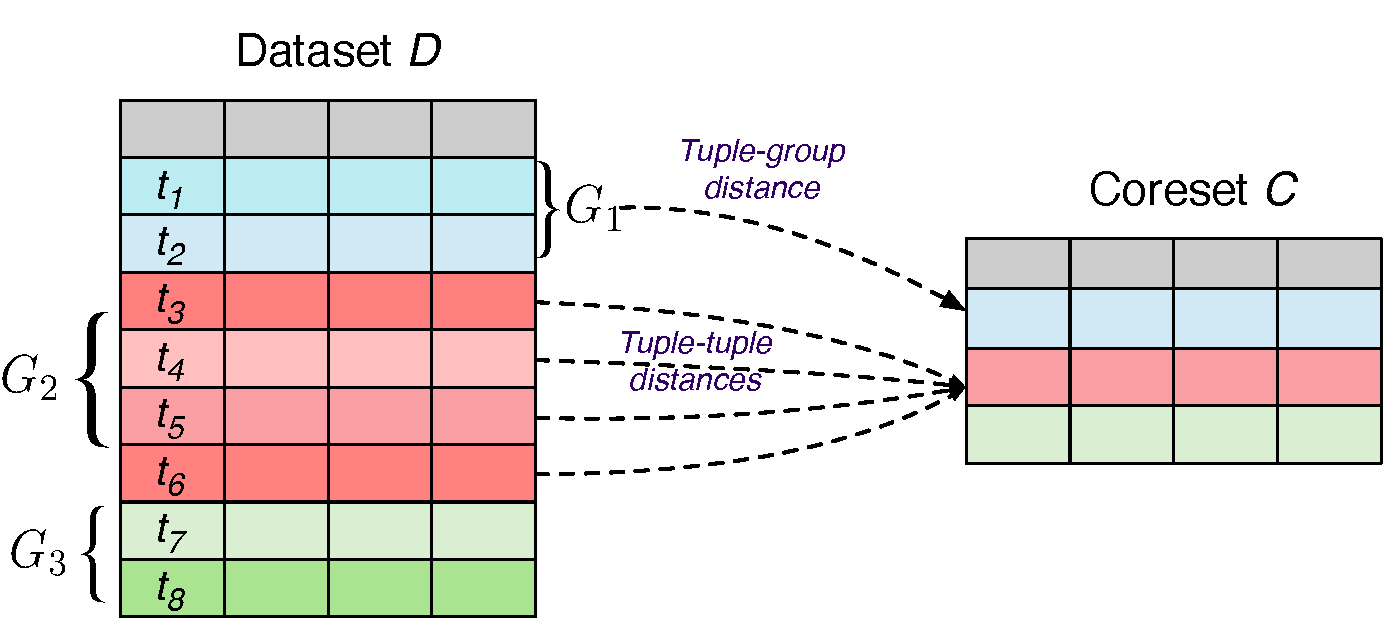
\includegraphics[width=0.6\textwidth]{figs/Overview-gb}
   % \vspace{-2.5em}
    \caption{Illustration of the Group-based Solution.}
    \label{fig:overview-gb}
   % \vspace{-1.5em}
\end{figure}

As shown in Figure~\ref{overview-gb}, one of the core parts of coreset computation is to compute the tuple-tuple distance, \ie $s_{ij}$. For the group-based solution, we just need to consider the relationship between tuples and these pre-computed groups, namely tuple-group distance, rather than the large amount of tuple-tuple distances. As we will discuss below, the computation of tuple-group distance does not need to iterate all tuples in the group, and thus  the overall efficiency can be much improved. 

At a high level, the overall process of group-based \ours solution with imputation in the loop is shown in Algorithm~\ref{alg:group}. To be more explicit, we illustrate Algorithm~\ref{alg:group} in comparison with Algorithm~\ref{alg:framework} in Section~\ref{subsec:framework} without clustering (the modified parts are highlighted in blue fonts).

To be specific, as shown in Line~\ref{alg4:cluster}, we first cluster $\trainc$ into groups using the efficient local sensitive hash (LSH) approach, where each group $\group_u, u\in[1, \groups]$ denotes the indexes of tuples in $\trainc$. In this way, every pair of tuples in the same group is close to each other in the feature distance.
%
 Afterwards, the major difference between group-based \ours and original \ours lies in the 3rd loop. Instead of  selecting a coreset to represent all tuples in the train set, group-based \ours selects a coreset to represent all clusters. As these clusters can well capture the train set distribution, the selected coreset contains enough information to approximate the full gradient of $\trainc$. 
 
 To this end, recap that the typical coreset selection algorithm needs the tuple-tuple distances to approximate the full gradient, while in group-based \ours, we just need to consider the tuple-group distances, \ie  
$\overline{s}_{\gamma(j)k} = \max\limits_{v \in \group_u} s_{\gamma(j)v}, s_{\gamma(j)v} = \lVert\mathbf{x}_v - \mathbf{x}_{\gamma(j)}\rVert, \gamma(j)\in[1, n]$, which denotes the maximum feature distance between the tuple $c_j$ in the coreset and all tuples in $\group_u$. As tuples in $\group_u$ are close to each other, $\overline{s}_{\gamma(j)k}$ can represent the relationship between $c_j$ and tuples in $\group_u$ to a large extent. But as shown in Line~11, we finally use an upper bound $\bound_{jk}$ to compute the coreset score because computing $\overline{s}_{\gamma(j)k}$ needs to iterate the tuples in $\group_u$, which is time-consuming. Next, we will theoretically show that using the upper bound can still derive a bounded GA error, leading to a well-performed coreset. 

%!TEX root = ../main.tex

\begin{figure}[!t]
 \vspace{-1em}
	\begin{algorithm}[H]
		\normalem
	\caption{Group-based \ours Solution (imputation-in-the-loop) \label{alg:group}}
		{\small
			
		\KwIn{Incomplete train data $\train$, coreset size $\numcore$, sample size $h$.}
		
		\KwOut{A coreset $\core \subseteq \train$, weight $\weightset=\{w_j\}$,$|\core|=|\weightset|=\numcore$.}
		
		$C=\emptyset$;\\\nllabel{alg1:init1}
		
		\add{Cluster $\train$ into groups $\groups = \{ \group_1, \group_2, ..., \group_\groupsize \}$;}\\\nllabel{alg4:cluster}
		
		\While{$|\core|< \numcore$}
		{\nllabel{craig1:loop1}
			
		/*1st loop*/  \\
		
		Sample $h$ tuples as $T_{sample} \subseteq \train \setminus \core$\\\nllabel{craig1:sample}
		
			\For{each tuple $t \in T_{sample}$}  
			{\nllabel{craig1:loop2}
				
				/*2nd loop*/ \\
				 $\hat{\core} = \core \cup \{t\}$;\\
			%	}
			 %$\mathrm{E}[t|\core]=\texttt{ComputeUtility}(t, C,D)$;
				 %/*3rd loop*/  \\\nllabel{craig1:loop3}
				 \For{\add{each group $G_k \in \groups$}}  
				 {
				 	\add{/*3rd loop*/} \\
				 
				 	%	Get the possible worlds of $\hat{\core} \cup \{t_i\}$;\\\nllabel{one:enumw}
				 	%	Compute $\mathrm{E}[\min_{c_j\in \hat{\core}}s_{ij}]$ using these possible worlds and their probabilities;\\\nllabel{one:exp4pw}
				 		\add{$\mathrm{E}[\hat{\core}] +\!\!= \mathrm{E}[\min_{c_j\in \hat{\core}}\bound_{jk} \times |\group_k|]$, where $\bound_{jk}$ is the upper bound of} \\\quad \\\nllabel{alg4:bound} \add{$\overline{s}_{\gamma(j)k} = \max\limits_{v \in \group_k} s_{\gamma(j)v}, s_{\gamma(j)v} = \lVert\mathbf{x}_v - \mathbf{x}_{\gamma(j)}\rVert, \gamma(j)\in[1, n]$; }\\\nllabel{one:dirtysum}
			     }
		         \add{$\mathrm{E}[t|\core] = \mathrm{E}[\core] - \mathrm{E}[\hat{\core}];$}
				 
			}		

			$t^*$ = $\argmax_{t\in T_{sample}}\mathrm{E}[t|\core]$ ;\\\nllabel{craig1:maxmulti}
			\If{$\mathbb{I}[t^*] = 1$} {\nllabel{craig1:oracle1}
				        Impute $t$ by a  human or automatic method.\\\nllabel{craig1:oracle}
				    }
			$\core = \core \cup \{t^*\}$;
			\\\nllabel{craig1:add2} 
			
				%\If{$\mathbb{I}[t^*] = 1$}
		%	{ \nllabel{alg:if}
		%		 \cc{Impute $t^*$ (by human or automatic methods).}\\\nllabel{alg:oracle}
		%	
			%}					
		}
	 %   \For{ $t\in \core$} 
	  %  {\nllabel{craig1:goodcore1}
	 %      \If{$\mathbb{I}[t] = 1$} {\nllabel{craig1:oracle1}
	 %        Impute $t$ by a  human or automatic method.\\\nllabel{craig1:oracle}
      %       }
     %   }
    
	 	\For{$j = 1$ to $|\core|$} 
	 	{\nllabel{craig1:cc0}
	 		%$w_j = \sum_{i=1}^{n}\mathbb{I}'[j=\argmin_{c_{j'}\in\core}  %\max\limits_{\hypo\in\vartheta}\lVert \df_i(\hypo) - \df_{\gamma(j')}(\hypo) \rVert ]$;\\\nllabel{craig1:cc}
	 		\For{$i = 1$ to n}
	 		{
	 		  \If{$c_j=\argmin_{c_{j'}\in\core}\max\limits_{\hypo\in\vartheta}\lVert \df_i(\hypo) - \df_{\gamma(j')}(\hypo) \rVert$}
	 		  {
	 		  	$w_j~+\!=~1$;\\\nllabel{craig1:cc}
	 		  }
 		    }
	 		
	 	}
		\Return $\core,\weightset$;\\\nllabel{craig1:return}
		}
	\end{algorithm}
\end{figure}




\subsection{Group-based GA Error Bound}

In this section, following the equations in previous sections, we deduce the GA error bound for our group-based solution. 
%
After clustering $\trainc$ to $\{ \group_1 , \group_2, ...\group_u\}$, considering Equation~\ref{eqa:tuple}, we  first rewrite the sum of $n$ feature distances (\ie $\min_{c_j\in \core_k}\lVert\mathbf{x}_i - \mathbf{x}_{\gamma(j)}\rVert$) to   $|\groups|$ summations. Each summation is the sum of $|\group_u|$ feature distances, as shown in the following Equation:
\vspace{-0.5em}
\begin{equation}\label{eqa:cluster-1}
 \mathrm{E}[C] = \sum_{k= 1}^{|\worlds|} p_k (\sum_{i=1}^n \min_{c_j\in C_k}\lVert\mathbf{x}_i - \mathbf{x}_{\gamma(j)}\rVert) =  \sum_{k= 1}^{|\worlds|} p_k (\sum_{u=1}^{\groups}\sum_{v \in \group_u} \min_{c_j\in C_k}\lVert\mathbf{x}_v - \mathbf{x}_{\gamma(j)}\rVert)
\end{equation}

Afterwards, as shown in Equation~\ref{eqa:cluster-2},  the sum of each cluster can be bounded by  the maximum distance ($\max_{v \in \group_u} \min_{c_j\in \core_k}\lVert\mathbf{x}_v - \mathbf{x}_{\gamma(j)}\rVert$)  multiplying the  cluster size, but the bound is expensive to compute because of iterating $\trainc$. To address this, we further apply the max-min inequality~\cite{} to simplify the computations. 


\begin{equation}\label{eqa:cluster-2}
\begin{aligned}
<<<<<<< HEAD
&  \sum_{k= 1}^{|\worlds|} p_k (\sum_{u=1}^{\groups}\sum_{v \in \group_u} \min_{c_j\in C_k}\lVert\mathbf{x}_v - \mathbf{x}_{\gamma(j)}\rVert) \\
& \leq \sum_{k= 1}^{|\worlds|} p_k (\sum_{u=1}^{\groups} |\group_u| \max_{v \in \group_u} \min_{c_j\in C_k}\lVert\mathbf{x}_v - \mathbf{x}_{\gamma(j)}\rVert) \\
&  \leq \sum_{k= 1}^{|\worlds|} p_k (\sum_{u=1}^{\groups} |\group_u| \min_{c_j\in C_k} \max_{v \in \group_u} \lVert\mathbf{x}_v - \mathbf{x}_{\gamma(j)}\rVert) \\
& =  \sum_{k= 1}^{|\worlds|} p_k (\sum_{u=1}^{\groups} |\group_u| \min_{c_j\in C_k} \overline{s}_{\gamma(j)v})
=======
  \sum_{k= 1}^{|\worlds|} p_k (\sum_{u=1}^{\groups}\sum_{v \in \group_u} &\min_{c_j\in C_k}\lVert\mathbf{x}_v - \mathbf{x}_{\gamma(j)}\rVert) 
 \leq \sum_{k= 1}^{|\worlds|} p_k (\sum_{u=1}^{\groups} |\group_u| \max_{v \in \group_u} \min_{c_j\in C_k}\lVert\mathbf{x}_v - \mathbf{x}_{\gamma(j)}\rVert) \\
 & \leq \sum_{k= 1}^{|\worlds|} p_k (\sum_{u=1}^{\groups} |\group_u| \min_{c_j\in C_k} \max_{v \in \group_u} \lVert\mathbf{x}_v - \mathbf{x}_{\gamma(j)}\rVert)
>>>>>>> 24f8f599829e50d52804de6e3863631109c36630
\end{aligned}
\end{equation}



Therefore,  we are able to iterate the much smaller cluster $\group$ to compute  the maximum feature distance (\ie $\overline{s}_{\gamma(j)k} = \max_{v \in \group_u} \lVert\mathbf{x}_v - \mathbf{x}_{\gamma(j)}\rVert, j \in [1,|\core_k|]$) between each $c_j \in \core_k$ and tuples in each cluster $\group_u$. Then, similar to assigning tuples of the full train set to the tuple of the coreset in previous sections, we can assign the cluster $\group_u$ to the tuple  with the minumum distance, \ie $\min_{c_j\in C_k} \overline{s}_{\gamma(j)v}$. To achieve efficient coreset selection, given $\trainc$ and clusters $\group$, we should precompute all the maximum feature distances $\{\overline{s}_{\gamma(j)k}|j \in [1,N], k \in [1,\groups]\}$. In this way, we can directly get the value of $\overline{s}_{\gamma(j)k}$. However, as discussed above, computing $\overline{s}_{\gamma(j)k}$ needs to visit every tuple in a cluster, which is still inefficient, so we  efficiently compute an upper bound $b_{jk}$ of  $\overline{s}_{\gamma(j)k}$ to replace $\overline{s}_{\gamma(j)k}$. Theoretically, following Eq.~\ref{eqa:cluster-1}, we have:
\vspace{-0.5em}
\begin{equation}\label{eqa:cluster-3}
    \begin{aligned}
        \sum_{k= 1}^{|\worlds|} p_k (\sum_{u=1}^{\groups} |\group_u| \min_{c_j\in C_k} \overline{s}_{\gamma(j)k}) \leq \sum_{k= 1}^{|\worlds|} p_k (\sum_{u=1}^{\groups} |\group_u| \min_{c_j\in C_k} b_{jk})
    \end{aligned}
\end{equation}

Similar to Sec~\ref{subsec:exp}, directly computing the probability and getting the expectation is extremely expensive, and thus we still can convert the expectation computation over the possible worlds associated with all clusters to the sum of expectation of each cluster, as follows:
\vspace{-0.5em}
\begin{equation}\label{eqa:cluster-4}
    \begin{aligned}
        \sum_{k= 1}^{|\worlds|} p_k (\sum_{u=1}^{\groups} |\group_u| \min_{c_j\in C_k} b_{jk}) = \sum_{u=1}^{\groups} \mathrm{E}[\min_{c_j\in \hat{\core}}\bound_{jk} \times |\group_u|]
    \end{aligned}
\end{equation}

\subsection{Algorithm Details}


\subsubsection{Clustering}
\label{subsec:clustering}
To cluster $\train$ efficiently,  we use the local sensitive hashing~\cite{} (LSH) to efficiently hash similar tuples to the same group.The basic idea  is to hash $\trainc$ with $r$ random hyperplanes $\{\mathbf{h}_1, \mathbf{h}_2, \dots, \mathbf{h}_r\}$ in the  $m$-dimensional space.Each hyperplane divides the entire space into two half subspaces, and LSH just hashes the  items according to which subspace they fall in. Specifically, for  hyperplane $\mathbf{h}_w, u\in[1,p]$, LSH hashes tuple $t_i\in \trainc$ to hash value 1 if $\mathbf{h}_w \cdot \mathbf{x}_i> 0$, and 0 otherwise.
In this way, each $t_i$ is hashed into a $p$-bit 0-1 hash code by $p$ hyperplanes.
Since the items with the same hash code are highly similar, we take them as a cluster.
Clustering by LSH is highly efficient as it has a complexity of  $O(Nrm)$, linear with $|\trainc|$. 

\subsubsection{Computing the upper bound}

Given an item $t_i\in \trainc$ and a cluster $\group_u \in \mathcal{G}$, recap that it is too expensive to  compute $\overline{s}_{\gamma(j)k}$, so we compute an upper bound $b_{jk}$. Next, we propose PQ-based solution to address this, which rely on the key idea that splits the $m$ dimension feature space into $M$ low dimensional subspaces. The feature vector $\mathbf{x}_i$ of  $t_i$ is also splitted into $M$ subvectors, each of which is denoted by $\mathbf{x}^a_i$. 
Then we respectively compute the upper bound of the maximum distance between $a$-th subvector and vectors of $m$-th feature subspace in $\group_u$, $a\in [1,M]$, and sum them up, producing the upper bound $b_{jk}$ between $t_i$ and $\group_u$. Formally, following Eq. ~\ref{eqa:cluster-3}, we have:

\begin{equation}\label{eqa:cluster-5}
    \begin{aligned}
    \sum_{u=1}^{\groups} |\group_u| \min_{c_j\in C_k} \max_{v \in \group_u} s_{\gamma(j)k} \leq\sum_{u=1}^{\groups} |\group_u| \min_{c_j\in C_k} \max_{v \in \group_u} s^a_{\gamma(j)v}
    \end{aligned}
\end{equation}

\noindent we use $s^a_{\gamma(j)v} = \max\limits_{v \in \group_u}\lVert \mathbf{x}^a_v - \mathbf{x}^a_{\gamma(j)}\rVert$ to denote the aforementioned maximum feature distance \wrt the $l$-th subspace. We can take $b_{\gamma(j)v}$ as $\sum_{a=1}^{M} s^a_{\gamma(j)v}$. To compute $b_{\gamma(j)v}$, next, we  discuss how to efficiently compute  $s^a_{iv}, i\in [1,N]$.

We first  introduce the basic concept of PQ widely used in the era of approximate nearest neighbor (ANN) search, which also uses the idea of  decomposing the entire feature space to a Cartesian product of subspaces with low dimensions~\cite{}. Each subspace is quantized separately. Hence, a feature vector can be represented as a short code, and the $a$-th element of the code denotes the  quantization index of the $a$-th subspace of the vector. Finally, in ANN search,  the Euclidean distance between two items can be efficiently estimated from their codes. Next, we will see how to leverage PQ to address our problem.

As shown  in Figure~\ref{}, given the full train data $\trainc$ with $m=$, suppose that we divide it into $M=$ subspaces, each of which has 2 dimensions (the upper left part of Figure~\ref{}).  For each subspace, we can sample some tuples and run $k-$means algorithm~\cite{} over this subspace. Suppose that $B$ denotes the number of clusters produced by $k-$means, so in Figure~\ref{}, $\{b_1^1, b_1^2,..., b_1^B\}$ denote the $k-$means cluster centers in the first subspace, associated with indexes (codes) $\{1, 2,...,B\}$. Then, a codebook $cb_1$ is computed, which records the feature distance between each pair of cluster centers, and we have $M$ codebooks in total (the lower left part of Figure~\ref{}). We use $cb_1[x][y]$ to denote the distance between the $x$-th and $y$-th centers. In this way, any $t_i (\mathbf{x}_i) \in \trainc$ can be quantized to a short code $c_i$ with length $M$, and we use $c_i^a, a\in[1,M]$  to denote the $l$-th code, which means the $c_i^a$-th center is the closest one to $\mathbf{x}_i^a$ among all clusters in the $a$-th subspace (the upper right part of Figure~\ref{}). For example, $c_i^1 =4$ because $b_1^4$ is the closest cluster with $\mathbf{x}_i^1$. For any $d_i, d_j$, their feature distance can be approximated by $s_{ij}=\sum_{l=1}^{M}cb_a[c_i^a][c_j^a]$. 



